\documentclass[conference]{../lib/IEEEtran}
\IEEEoverridecommandlockouts
% The preceding line is only needed to identify funding in the first footnote. If that is unneeded, please comment it out.
\usepackage{cite}
\usepackage{amsmath,amssymb,amsfonts}
\usepackage{algorithmic}
\usepackage{graphicx}
\usepackage{textcomp}
\usepackage{xcolor}
\def\BibTeX{{\rm B\kern-.05em{\sc i\kern-.025em b}\kern-.08em
    T\kern-.1667em\lower.7ex\hbox{E}\kern-.125emX}}

\usepackage{minted}

\usepackage[per-mode=symbol,input-symbols=w_1]{siunitx}
\DeclareSIUnit\sample{samples}
\DeclareSIUnit\width{widths}
\DeclareSIUnit\digit{digits}
\DeclareSIUnit\uend{ends}
\DeclareSIUnit\separator{separator}

\usepackage{nonfloat}
\renewenvironment*{figure}[1][]
    {
        \minipage{\linewidth}
    }
    {
        \endminipage
        \\*[\intextsep]
    }
\renewenvironment*{table}[1][]
    {
        \minipage{\linewidth}
    }
    {
        \endminipage
        \\*[\intextsep]
    }
%--------------------------------------------------

\usepackage{mathtools}%
\DeclarePairedDelimiter\abs\lvert\rvert%
\DeclarePairedDelimiter\brao()%
\DeclarePairedDelimiter\brac[]%
\DeclarePairedDelimiter\braco[)%
\DeclarePairedDelimiter\braoc(]%
\DeclarePairedDelimiter\Brac\{\}%
\DeclarePairedDelimiter\angl<>%
\DeclarePairedDelimiter\floor\lfloor\rfloor%
\DeclarePairedDelimiter\piece\{.%

\newcommand*\hfrac[2]{#1/#2}
\newcommand*\tbrao[1]{(#1)}

\begin{document}

\title{ECE 4522 MATLAB Assignment 2}

\author{\IEEEauthorblockN{Leomar Dur\'an}
\IEEEauthorblockA{\textit{College of Engineering} \\
\textit{Temple University}\\
Philadelphia, PA \\
leomar.duran@temple.edu}
}

\maketitle

\begin{abstract}
This assignment introduces the backward difference system, and uses cascading to produce an edge detector. This works because the difference of the current value and the previous are zero if they were equal, and larger if they are more different. The backward difference system is produced in 3 steps, and is first tested. We finally apply the edge detector to a photograph of a barcode to prepare it for decoding.
\end{abstract}

\begin{IEEEkeywords}
convolution, filter, backward difference system, difference system, edge detection, threshold, barcode, encode, decode
\end{IEEEkeywords}

\section{Objectives}

The objectives of this report is to show the use of a backward difference system, implement an edge detection filter and use this filter to read a barcode.

After this lab, students will be able to apply a difference system, and explain what it does.

\section{Methods}

\mintinline{bash}{./Ece4522/MatlabAssignment3/B1.m} demonstrates and tests the first \(3\) steps of the edge detection filter. More specifically, it
\begin{enumerate}
    \item
        creates a sample signal, a square wave with a \(10\)-sample duty cycle, a period of \(30\) samples, and an amplitude of \(255\).
    \item
        uses the backward difference system modeled by \tbrao{\ref{eqn:bdn}} to find the edges of the sample signal, where its value changes.
        \begin{eqnarray}\label{eqn:bdn}
            y\brac{n} := x\brac{n} - x\brac{n - 1}.
        \end{eqnarray}
    \item
        checks the absolute value of this resulting signal against a \(\SI{60}\percent\) tolerance to create a sparse location signal.
    \item
        compresses the location signal by removing all \textsc{zero} values using the \mintinline{matlab}{find()} function.
\end{enumerate}

Rather than using a sample signal, \mintinline{bash}{./Ece4522/MatlabAssignment3/B2.m} first reads from a photo of a barcode, and samples the middle row as the input signal.

After compressing the location signal,
\begin{enumerate}
    \item
        the signal is once again pass through a backward difference system.
    \item
        the values of this signal are then regularized to between \(1\) and \(4\) by dividing by the base width for that \(59\)-edge interval.
    \item
        finally, the first end code 1-1-1 is located, and the next \(59\) values from and including that end point are cut out and decoded.
\end{enumerate}

\section{Results}

\subsection{Part B.1 Edge Detection and Location in 1-D Signals}

\begin{figure}
    \centering
    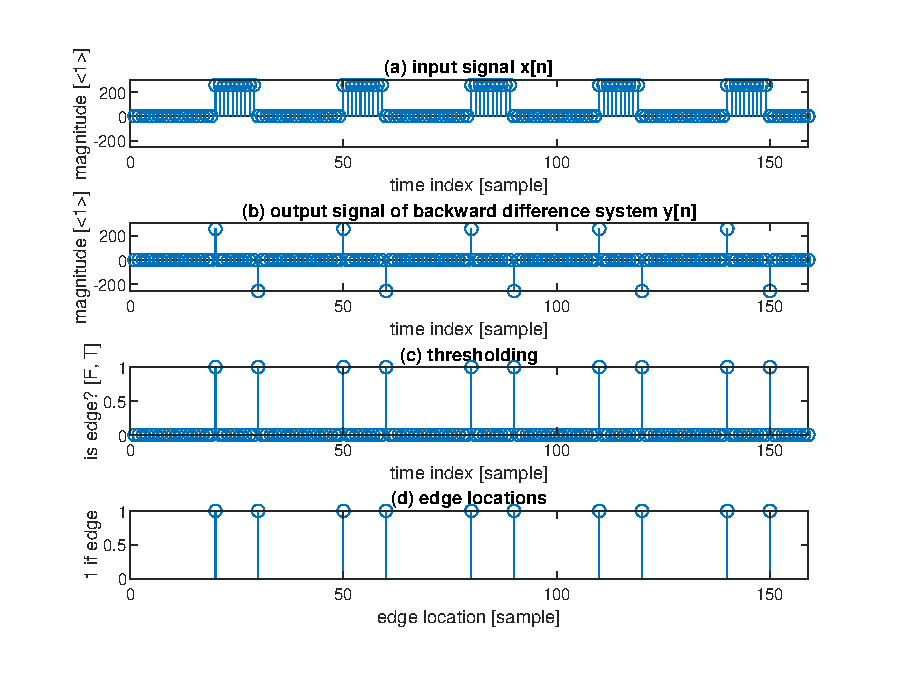
\includegraphics[width=\linewidth]{ece4522ma3fig1.eps}
    \figcaption{(a) the input square wave signal, (b) the result of the backward difference system, (c) the result of thresholding by checking the absolute value against a \(\SI{60}\percent\) tolerance, and (d) the output compressed edge locations.}
    \label{fig:B.1-fig1}
\end{figure}

\subsection{Part B.2 Bar Code Detection and Decoding}

\begin{figure}
    \centering
    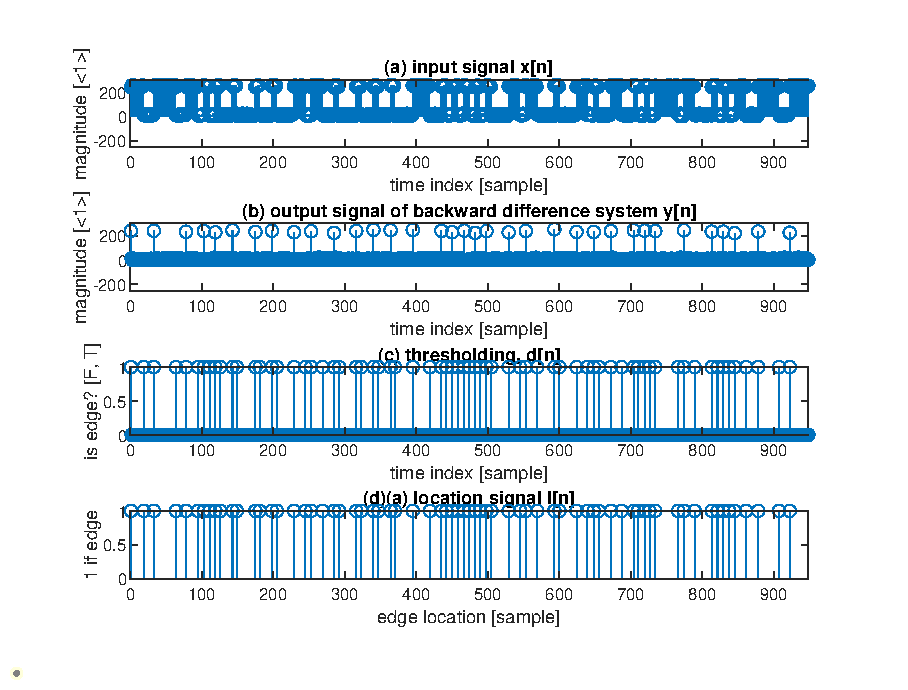
\includegraphics[width=\linewidth]{ece4522ma3fig2.eps}
    \figcaption{(a) the input square signal read from the barcode image, (b) the result of the backward difference system, (c) the result of thresholding by checking the absolute value against a \(\SI{60}\percent\) tolerance, and (d) the output compressed edge locations.}
    \label{fig:B.2-fig2}
\end{figure}

\begin{figure}
    \centering
    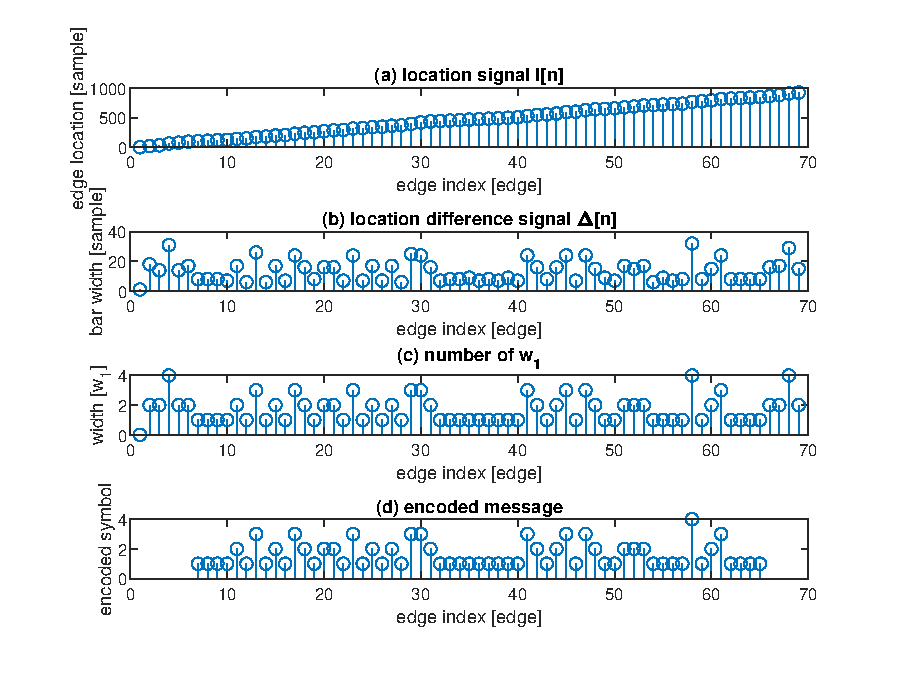
\includegraphics[width=\linewidth]{ece4522ma3fig3.eps}
    \figcaption{(a) the location signal, (b) the result of running the location signal through the backward difference system, (c) \(\Delta\brac{m_0, n}\) in terms of \(w_1\) and (d) the cropped out message from part (c).}
    \label{fig:B.2-fig3}
\end{figure}

The results of \mintinline{bash}{./Ece4522/MatlabAssignment3/B1.m} show
\begin{minted}{matlab}
decodeMessage =

     8     8     2     7     8     0     4
     5     0     1     6     5
\end{minted}

These were the digits expected from the original barcode.

\section{Insights}

\subsection{Part B.1 Edge Detection and Location in 1-D Signals}

The signal in Fig. \ref{fig:B.1-fig1}(b) is created by subtracting the present value of \(x\brac{m_0, n}\) in part (a) from its value \(1\) sample ago as represented by \tbrao{\ref{eqn:bdn}}. This has the result of \textsc{zero}ing out in \(y\brac{m_0, n}\) where \(x\brac{m_0, n}\) is flat because these values are constant, and the difference between a constant and itself is \textsc{zero}. It also emphasizes edges because their result is non-\textsc{zero}. These appear as impulses. They are positive impulses when the \(x\brac{n} > x\brac{n - 1}\) and negative impulses when \(x\brac{n} < x\brac{n - 1}\).

Along with the thresholding in Fig. \ref{fig:B.1-fig1}(c), this marks the edge immediately after the transition because of the reference to \(x\brac{n - 1}\).

\subsection{Part B.2 Bar Code Detection and Decoding}

Since \(\Delta\brac{m_0, n}\) represents the differences in the locations of edges, the vertical axis in Fig. \ref{fig:B.2-fig3} shows the width of the bar enclosed by those edges. Ignoring the first \textsc{zero} height, we can see \(4\) distinct heights of approximately \(8.2, 16.4, 24.6\), and \(32.8\) \si\sample.

Now we can justify that the total width of a signal is \(95\) times the base width of the shortest bar. This is because there are \(12\) digits each with width \(7\), \(2\) end delimiters of width \(3\), and 1 middle separator of width \(5\). So the message is \(\brao{\SI{12}\digit \times \SI{7w_1}{\per\digit}} + \brao{\SI{2}\uend \times \SI{3w_1}{\per\uend}} + \brao{\SI{1}\separator \times \SI{5w_1}{\per\separator}} = 95w_1\). Also, from part \textbf{B.2} of the lab manual, we know to expected \(59\) bars in the barcode message. Thus, we can expect any interval of \(59\) bars to be of size \(95w_1\). By dividing these by \(95\), we find the base width of the thinnest bar \(w_1\).

\section{Conclusion}

We have implemented and tested a backward difference system. Then we have shown how two backward difference systems can be used to implement an edge detection system, and further used that edge detection system to help decode a barcode.

As the resulting value of \mintinline{matlab}{decodeMessage} shows, we were successfully able to find the encoded message in the photograph of the barcode.

\end{document}
